Whenever the heavy ion collision reaches a new high energy, the first thing to check is the energy dependence of the flow harmonics. ALICE has published the measurement of $v_2$ at 5.02 TeV Pb+Pb and compared with previous energies~\cite{Adam:2016izf}, as shown in Fig.~\ref{fig:result_energyDep_ALICE}. Except for the lowest energies, where $v_2$ could go negative, for $\sqrt{s_\text{NN}}>5$ GeV, as the collision energy increases, the $v_2$ also increases. At the TeV level, the magnitude of $v_2$ almost saturates.
\begin{figure}[H]
\centering
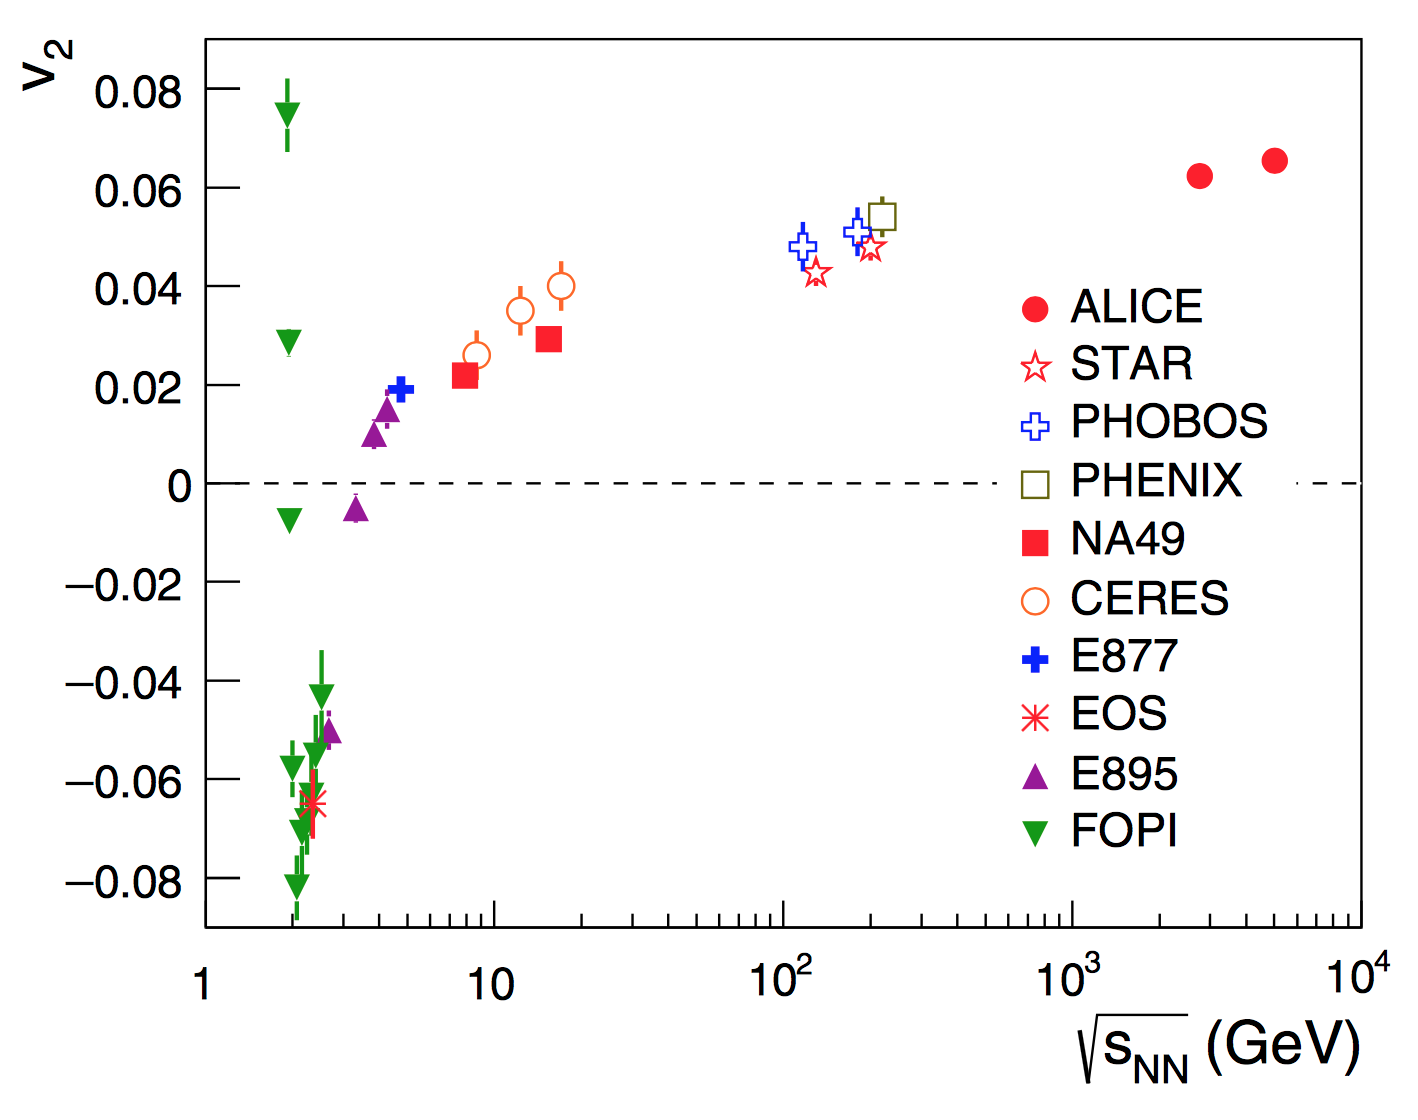
\includegraphics[width=.7\linewidth]{figs/sec_result/energyDep_ALICE.png}
\caption{$v_2$ measured as a function of different collision energies $\sqrt{s_\text{NN}}$, published by ALICE.}
\label{fig:result_energyDep_ALICE}
\end{figure}

ATLAS has measured the $p_\text{T}$ dependence of $c_2\{4\}$ and $c_3\{4\}$ with 2.76 TeV Pb+Pb data~\cite{ATLAS:2014vba}, as shown in Fig.~\ref{fig:result_v2v3_pT_ATLAS}. For $v_2\{2\}$ and higher order cumulants, the magnitude of $v_2$ first increases with $p_\text{T}$, reaches maximum around $2-3$ GeV, then decreases as $p_\text{T}$ goes even higher.
\begin{figure}[H]
\centering
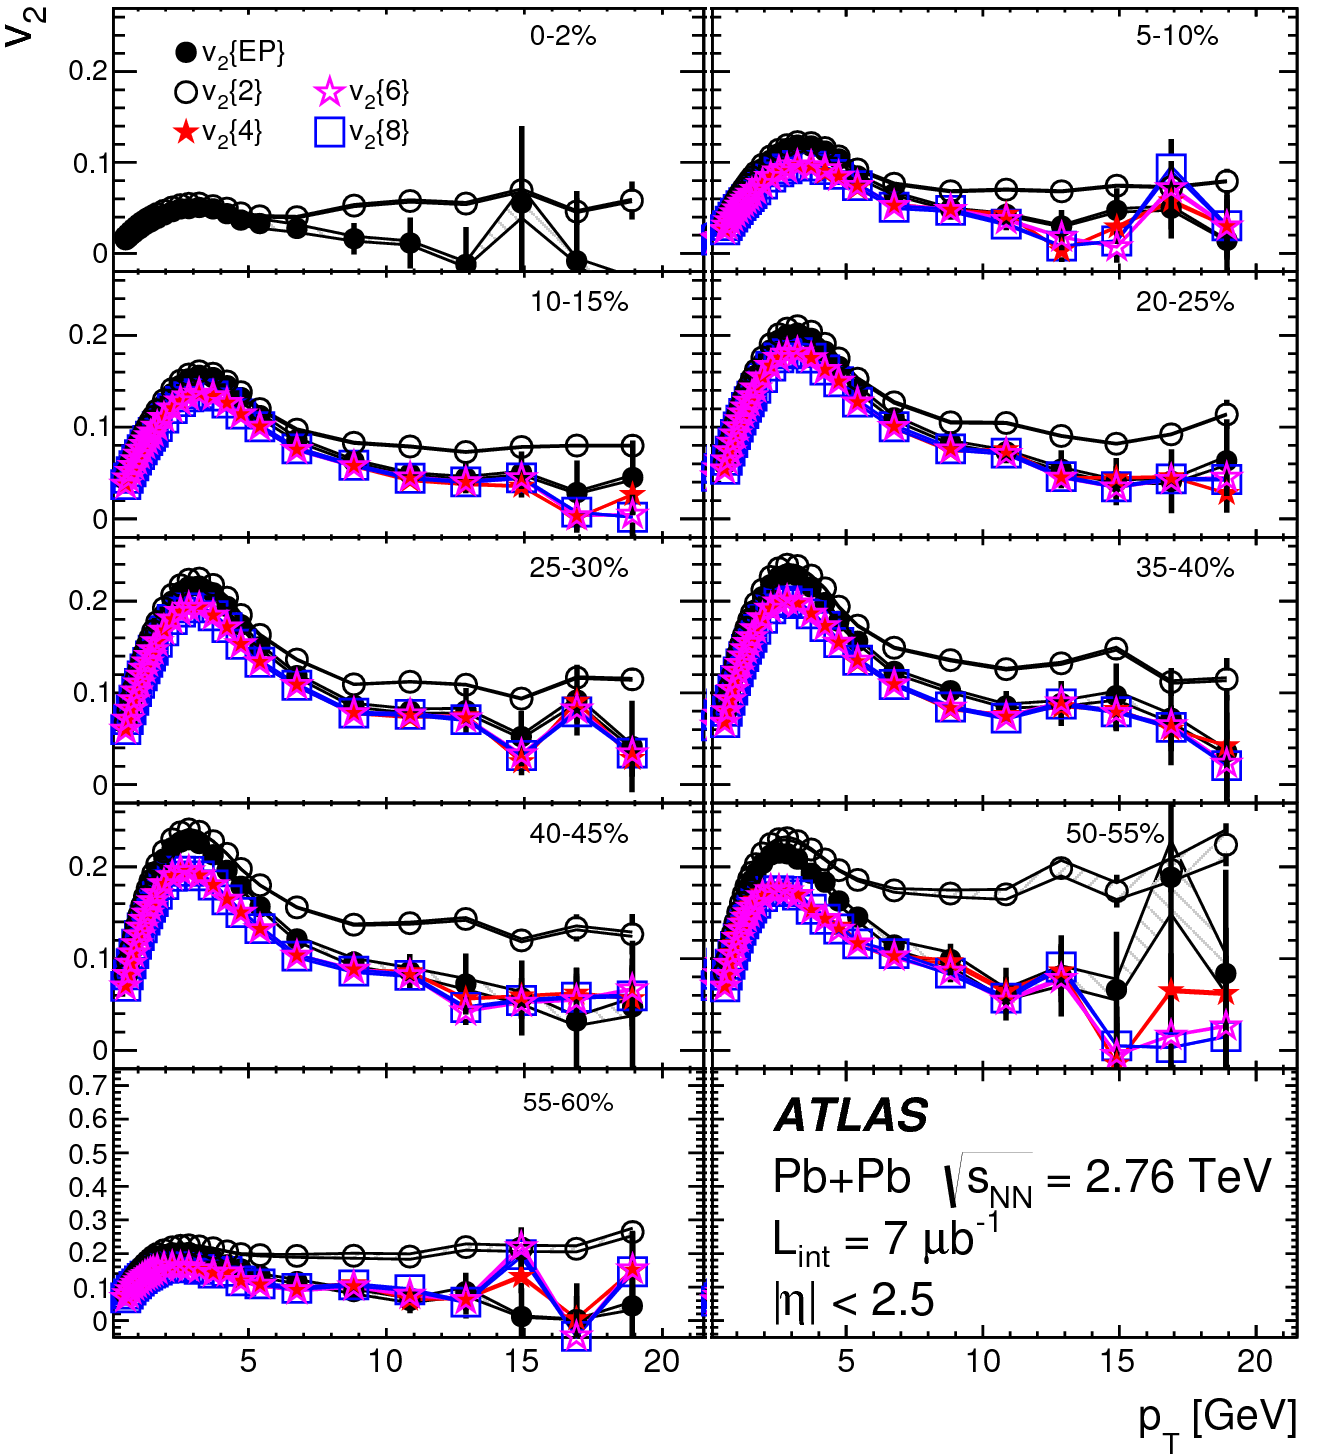
\includegraphics[width=.75\linewidth]{figs/sec_result/v2v3_pT_ATLAS.png}
\caption{$v_2\{2k\}$ measured as a function of $p_\text{T}$, published by ATLAS}
\label{fig:result_v2v3_pT_ATLAS}
\end{figure}

Note that in previous differential multi-particle cumulant measurements~\cite{Aad:2014vba}, $p_\text{T}$ dependence are measured with respect to only one reference particles. While in this analysis, the $p_\text{T}$ dependence are measured with all the particles. For example, to measure cumulant $c_2\{4\}$ in range $2.0<p_\text{T}<5.0$ GeV:
\begin{itemize}
\item Previous differential cumulant: in $\lr{e^{in(\phi_i+\phi_j-\phi_k-\phi_l)}}$, only one particle is from $2.0<p_\text{T}<5.0$ GeV and the rest three particles are from $0.5<p_\text{T}<5.0$ GeV;
\item This analysis: in $\lr{e^{in(\phi_i+\phi_j-\phi_k-\phi_l)}}$, all the four particles are from $2.0<p_\text{T}<5.0$ GeV;
\end{itemize}
The previous differential cumulant measurement assumes that the flow in different $p_\text{T}$ ranges share the same event plane, which might not be the case as shown by the flow decorrelation measurement in $p_\text{T}$~\cite{Khachatryan:2015oea}. Note that there also exists decorrelation in $\eta$~\cite{Aaboud:2017tql}, but in this analysis we are only measuring cumulants as a function of $p_\text{T}$. With Run 2 Pb+Pb data, the statistics are higher, we are correlating all the particles in the selected $p_\text{T}$ range, instead of correlating particles from the low $p_\text{T}$ with high $p_\text{T}$. This will also benefit us in the way that the cumulant formulas are simpler than differential cumulant, without special treatment of reference particles.

For the measurement of $v_1$, a primary background is global momentum conservation (GMC), which induces a significant dipole component. ATLAS has published the 2-particle correlation measurement of $v_1\{2\}$ at 2.76 TeV Pb+Pb~\cite{ATLAS:2012at}, with momentum conservation effects properly removed, as shown in Fig.~\ref{fig:result_v1_pT_ATLAS}. $v_1\{2\}$ as a function of $p_\text{T}$ starts from negative values, and crosses 0 at $p_\text{T}~1$ GeV. It reaches maximum positive at $p_\text{T}~4$ GeV and then decreases towards very high $p_\text{T}$. Different centralities are shown in different panels, and the trends are very similar, meaning a weak centrality dependence of $v_1\{2\}$. Unlike 2-particle correlation, global momentum conservation does not play a role in 4-particle correlation. This is because the 4-particle cumulant is defined as:
\begin{equation}
c_1\{4\} = \lr{v_1^4} - 2\lr{v_1^2}^2
\end{equation}
where GMC contributes to both $\lr{v_1^4}$ and $\lr{v_1}^2$, then most of the effects are canceled.

But in order to obtain a non-zero $c_1\{4\}$ signal, the lowest $p_\text{T}$ cut at least needs to be above 1 GeV. Due to this reason, we have different lowest $p_\text{T}$ cuts from 1.0 GeV to 2.0 GeV.
\begin{figure}[H]
\centering
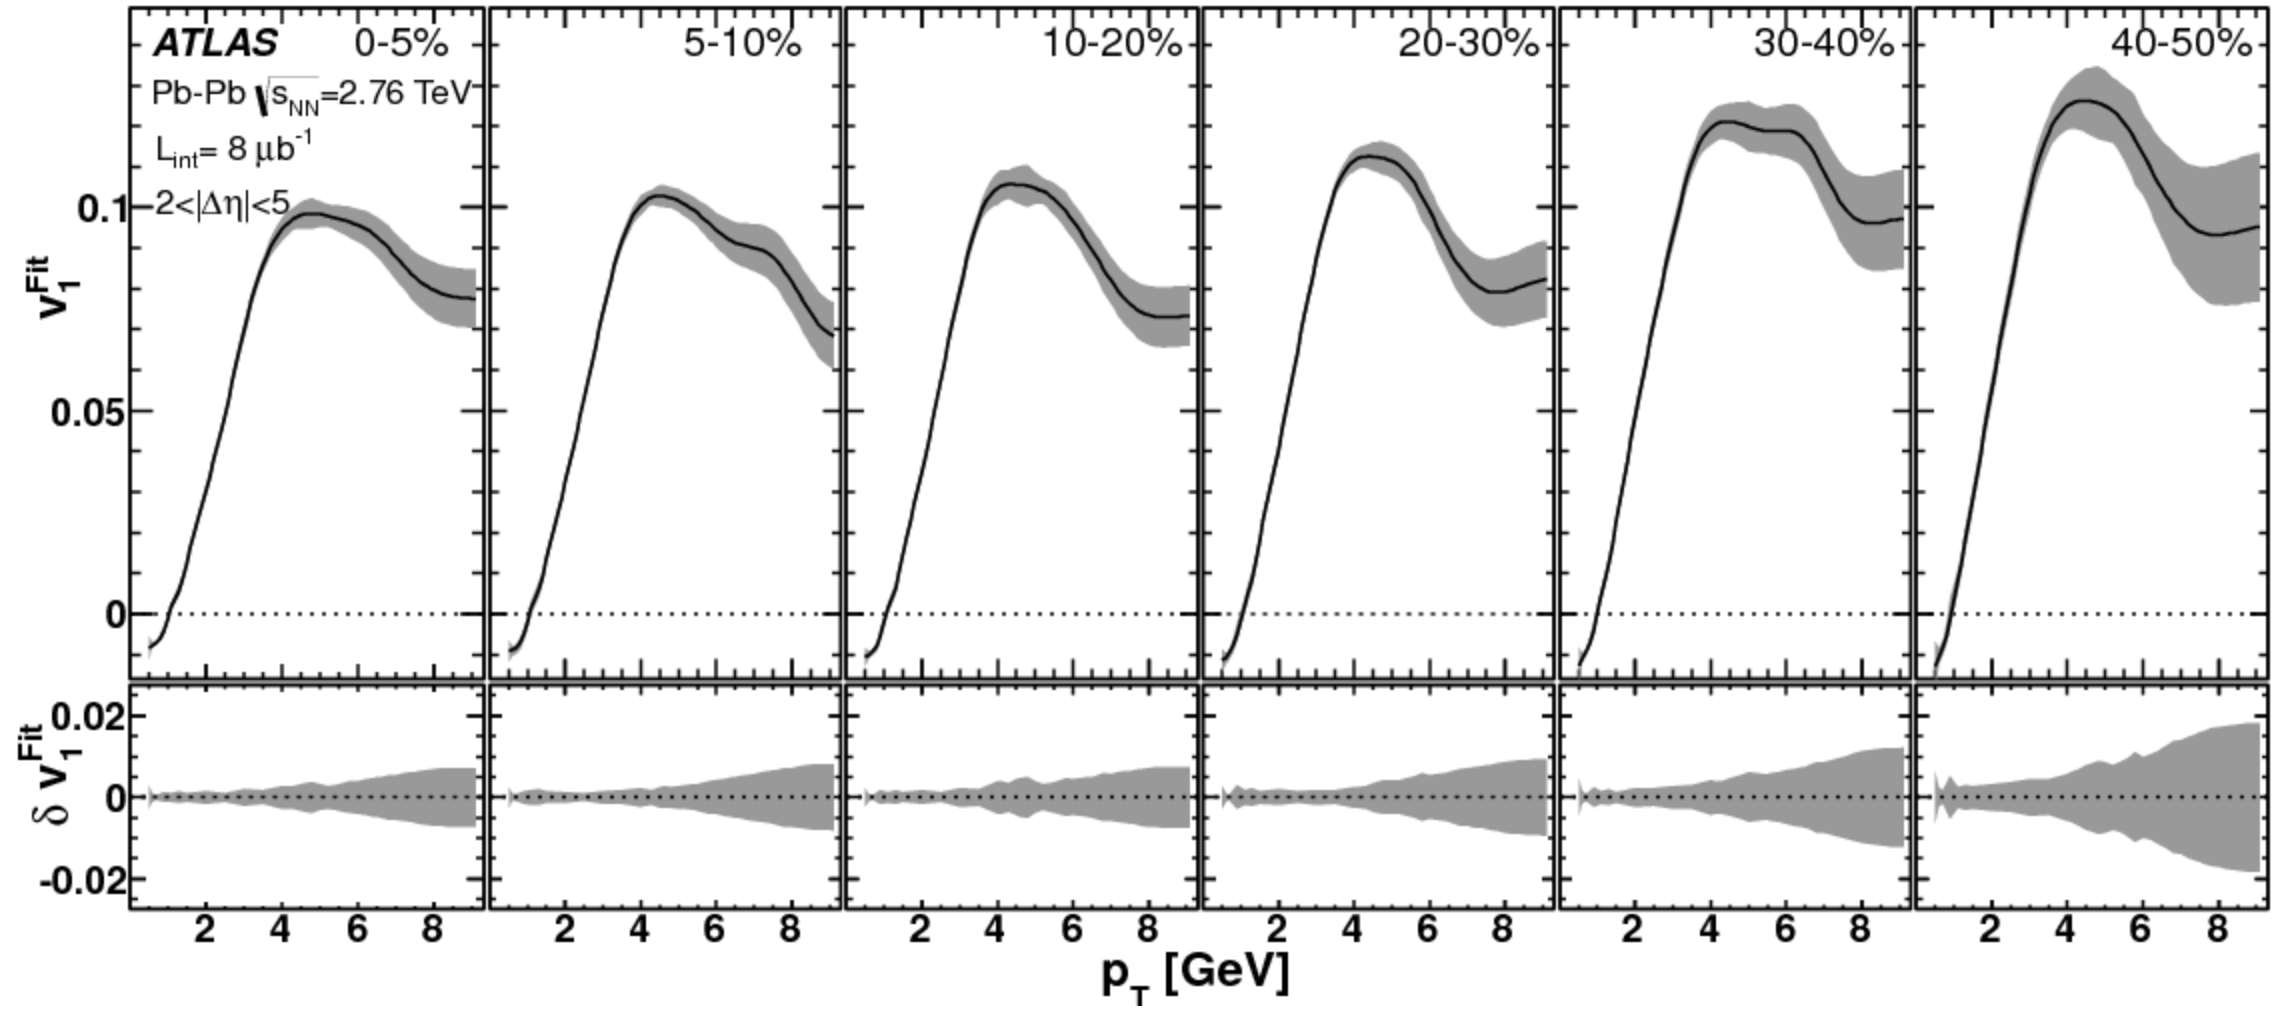
\includegraphics[width=.9\linewidth]{figs/sec_result/v1_pT_ATLAS.png}
\caption{$v_1\{2\}$ measured as a function of $p_\text{T}$, in different centralities, published by ATLAS.}
\label{fig:result_v1_pT_ATLAS}
\end{figure}

Symmetric cumulants, $sc_{n,m}\{4\}$, was first proposed and measured by ALICE~\cite{ALICE:2016kpq}, as shown in Fig.~\ref{fig:result_sc_ALICE}. Symmetric cumulants in HIJING are found to be consistent with 0, meaning that these observables are not sensitive to the non-flow contributions. In this analysis, we have extended the measurements to 5.02 TeV Pb+Pb, with multiple $p_\text{T}$ cuts. Both the energy of $p_\text{T}$ dependence of symmetric cumulants will provide more insights into the flow correlations.
\begin{figure}[H]
\centering
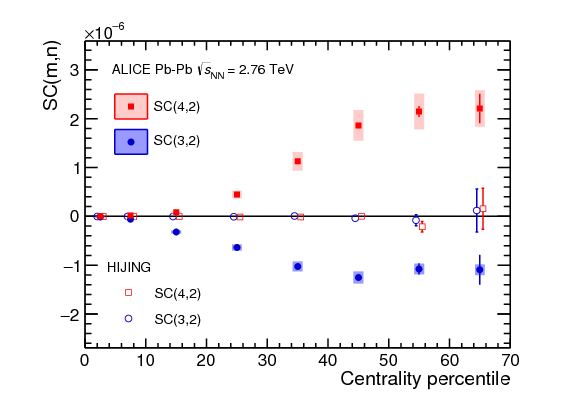
\includegraphics[width=.5\linewidth]{figs/sec_result/sc_ALICE.png}
\caption{Symmetric cumulants $sc_{2,3}\{4\}$ and $sc_{2,4}\{4\}$ as a function of centrality, measured by ALICE.}
\label{fig:result_sc_ALICE}
\end{figure}

Cumulant ratios have long been used to probe the fluctuation of eccentricity $\epsilon_n$ in the initial stage. Recently, CMS collaboration has published the non-Gaussian elliptic-flow fluctuation in 5.02 TeV Pb+Pb~\cite{Sirunyan:2017fts}. In the paper, they measured the cumulant ratio $v_2\{6\}/v_2\{4\}$, as shown in Fig.~\ref{fig:result_cr_CMS}, and the method they used the unfolding technique. In this analysis, we calculated the same observable using multi-particle cumulant. One advantage of cumulant method is that the systematics partially cancels in the ratio, which results in a much better precision. Furthermore, we have tested the non-Gaussian fluctuation in different $p_\text{T}$ ranges, which reflects the additional dynamical fluctuation after the initial stage.
\begin{figure}[H]
\centering
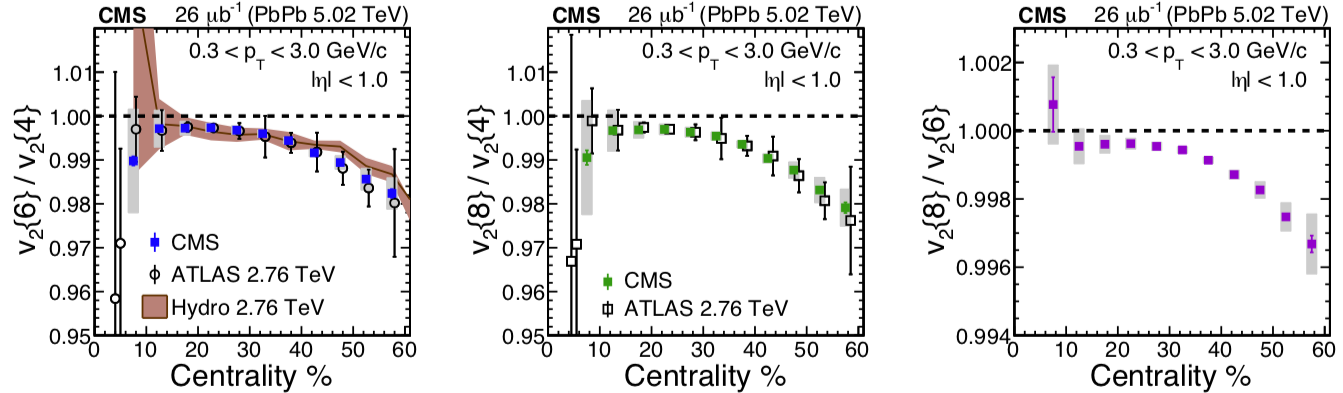
\includegraphics[width=.9\linewidth]{figs/sec_result/cr_CMS.png}
\caption{Cumulant ratio $v_2\{6\}/v_2\{4\}$ as a function of centrality, with unfolding method, published by CMS.}
\label{fig:result_cr_CMS}
\end{figure}







